\documentclass{article}
\usepackage[backend=biber,style=ieee]{biblatex}
\addbibresource{sources.bib}

\usepackage{color}
\usepackage{placeins}
\usepackage{listings}
\usepackage{graphicx}
\usepackage{xcolor}
\usepackage{amsmath}
\usepackage{subcaption}
\usepackage{cleveref}
\usepackage{array}
\usepackage{geometry}[margins=1in]
\setlength{\parskip}{4pt plus 2pt}
\setlength{\parindent}{0pt}
%\pagecolor[rgb]{0,0,0} %black
%\color[rgb]{1,1,1} %grey
\lstset{language=C++,
keywordstyle=\color{blue},
stringstyle=\color{red},
commentstyle=\color{green},
morecomment=[l][\color{magenta}]{\#},
breaklines=true,
breakatwhitespace=true,
numbers=left
}
\title{3-Dimensional Heisenberg Model}
\author{Asbjørn Bonefeld Preuss \and Daniel Lomholt Christensen \and Elie Cueto \and Frederik Aaboe Andersen \and Emilie Berg \and Nete Wen Yu O. Lyndrup}
%\affiliation{Niels Bohr Institute}
\date{March 2024}

\renewcommand{\vec}{\mathbf}
\usepackage{titlesec}
\titleformat{\section}
  {\normalfont\Large\bfseries}{Section \thesection}{1em}{}


  
\begin{document}
\maketitle
\renewcommand{\thepage}{}
\setcounter{page}{0}
\tableofcontents
\newpage
\renewcommand{\thepage}{\arabic{page}}
\section{Introduction}
This project seeks to implement the three-dimensional Heisenberg model into C++, and attempt to optimize the implementation, to allow simulations of larger systems, faster.

The project therefore starts with an Introduction to the Heisenberg model, followed by an overview of a sequential implementation, and then the parallelization that will be used to optimize the sequential implementation. Finally, a chapter showing the weak and strong scaling of the different versions, as well as profiling of the versions are presented.

\subsection{The Heisenberg Model}
The goal of the Heisenberg model is to predict the behavior of condensed matter systems.
The Heisenberg model assumes an N$\times$N$\times$N cube, occupied by N$\times$N$\times$N spins. These spins are vectors that can point in any direction in 3-d space. Each of these spins are generated as a random spin vector initially. 

Then the Metropolis-Hastings Monte Carlo algorithm is used\autocite{sneppenComplexPhysics2023}. This algorithm selects a random site and flips it in a new, random direction. If the flip minimizes the energy of the system, it is accepted. If not, a flip probability is calculated. This probability is $P=\exp\left(-\frac{\Delta E}{k_bT}\right)$ according to Boltzmann statistic \autocite{simonOxfordSolidState2013}.
A random number is then generated. If the random number is smaller than the probability, the flip is accepted. Otherwise, the flip is rejected, and the system remains the same.

The energy of the system is calculated by the Hamiltonian considering the 6 nearest neighbors of the spin as well as the strength and direction of the magnetic field \cite{simonOxfordSolidState2013}, cf. \cref{Hamiltonian}.
\begin{equation}
    H = - \frac{J}{2}\sum_{n, \lambda}\mathbf{S}_n\cdot\mathbf{S}_{n + \lambda} + g\mu_B\sum_n \vec{S}_n \cdot \vec{B}.
    \label{Hamiltonian}
\end{equation}
Here $g\mu_B$ are the gyromagnetic ratio and the Bohr magneton, which for the purpose of these calculations are set to unity.
At each flip, the energy of the old spin and new spin must be calculated according to \cref{Hamiltonian}. 

\section{Sequential Implementation} \label{sec:seq_imp}
The initial implementation first creates a class \verb|spin_system|, most importantly containing a (standard) vector of vectors of positions and a vector of vectors of spins, which are both initially empty. Two generator functions are then called that create the positions of the spins and the spin vectors. After this, another generator finds the indices of each spin's neighbors in all directions.

Then the simulation begins. A random site is chosen (seeded by index of the currently running iteration), and the energy of the current system, as well as the old spin state, is recorded. The new spin direction is calculated, as well as put directly into the system of spins, and its energy is found - each spin is set to have six neighbors that influence the mentioned. The two energies are compared. If the new energy is lower, the spin-flip is accepted. If the new energy is higher, the critical probability of acceptance is calculated. A random number (seeded by twice the iteration it is) is found. If the random number is larger than the critical probability, the change is not accepted and the old state of the spin is restored. This is done \texttt{flip} times, as requested in the command line. Our goal is to perform the simulation until convergence of the system (for temperatures below the critical temperature). We have applied a weak external B-field to the system that points in the z-direction. So we can check if the system has converged by checking that the magnetization of the system is parallel to the external B-field.

We expect the sequential version to be very slow for large system sizes since the single processor has to run through every single spin in the system for each time step in the simulation. Therefore, it is beneficial to exploit the potential parallelism in the problem and thereby speeding up the simulation which is the topic of the next sections.

\section{Parallelization}
There are two versions of the parallelization of the program. In both versions, 3-dimensional domain decomposition with distributed memory is used, and the Message Parsing Interface\autocite{mpi41}, \texttt{MPI}, is used for ghost cell communications between neighboring domains. The 3D global system is divided into 3D local subsystems, and each rank is assigned to a local system. There is given a set number of flips to simulate the global system, where each local system has to run $\frac{flips}{\#ranks}$ number of iterations. All ranks start by exchanging the edge of their domain with their neighbors (these are the ghost cells) with a \texttt{MPI\_Neighbor\_alltoallw}. The exchange of ghost cells is necessary since the calculation of the energy difference for two different states uses the nearest neighbors of the spins. So when a spin is flipped at the edge of a local system, the globally adjacent spins which belong to another local system needs to be known.

In version one, with each iteration, the ranks do the flipping in their local systems as in \cref{sec:seq_imp} and regardless of whether something flipped or not, and regardless of whether the flipped spin is at the local domain's edge or not, the ranks will send an "entire wall" of ghost-cells to its neighbors with \texttt{MPI\_Neighbor\_alltoallw}. This works, but it is not the most efficient way to exchange ghost cells. This is because it is only when a spin somewhere on the edge of a local domain is flipped that the neighbor's ghost cells need updating. If a spin is flipped in the interior of a local domain or if a proposed flip at the edge is rejected, then the neighboring domain will receive the same ghost cell values that it already has.

In version two we have implemented a different way to exchange ghost cells that does not have the inefficiency of version 1. With each iteration, a rank wants first to check if its neighbor has sent it anything, here \texttt{MPI\_Iprobe} is called. If the flag is output from \texttt{MPI\_Iprobe}, the rank shall use \texttt{MPI\_Recv}, which is a blocking receive, such that it can update its ghost-cells. \texttt{MPI\_Iprobe} is used to avoid putting a lot of non-blocking receives that may not need to receive as the edges of the neighboring ranks do not flip often for bigger systems.

A rank can now choose a random spin and do the flipping as explained in \cref{sec:seq_imp}. If a flip is performed at the edge, the rank sends non-blocking -- by \texttt{MPI\_Isend} -- \textit{only} the information of the given changed spin to the neighbors' ghost cells - not the whole "wall" as in version 1, and only to the neighbors that need it. An \texttt{MPI\_Barrier} is placed to ensure that the iteration is done before continuing to the next iteration. This is to prevent race conditions. Another barrier is also added to ensure that all ranks are done with their job for the current time step before starting the next. This is done in both versions and is to prevent some ranks coming ahead of other ranks.

Lastly, for both versions when the simulation is done, all local systems are gathered on rank 0 with \texttt{MPI\_Gather}. This way we end up with the global system.

Using this approach, it is possible to do as many flips at a time as there are ranks, in theory converging much faster even though an extra overhead is added.

\section{Results from simulations}
We have run the simulation for multiple temperatures and two different system sizes ($\#spins=729$ and $\#spins=27000$). For this, we used version 2 of the parallel implementation with 27 processors. From this we obtain data for energy, magnetization, etc. This data is investigated in this section. As a cross check we have also plotted data from the sequential version of the code for the small system. It should be noted that the temperature is in all cases in units of the Boltzmann's constant, $k_B$.  

\subsection{Energy}
We can find the total energy per spin from
\begin{equation}
    E = \frac{\sum{E_{j}}}{\#spin},
\end{equation}
where $j$ runs over each spin. In \cref{fig:energy}, we have visualized the total energy per spin as a function of temperature. Our program outputs the energy of each spin for the last iteration where the program has reached convergence for temperatures below the critical temperature. As expected, we see the lowest energies for the lowest temperatures, and the energy gradually rises as the temperature rises. For higher temperatures, the energy is close to 0. This is expected since these temperatures are above the critical temperature meaning that the system cannot converge so here the spins point in random directions in the system which sets the energy to zero. Furthermore, we see that the data from the sequential version of the program follows the same trend as the parallel version within any fluctuations that is expected due to the stochastic nature of the spin flipping. This supports the correctness of our parallel implementation.

\begin{figure}[ht!]
    \centering
    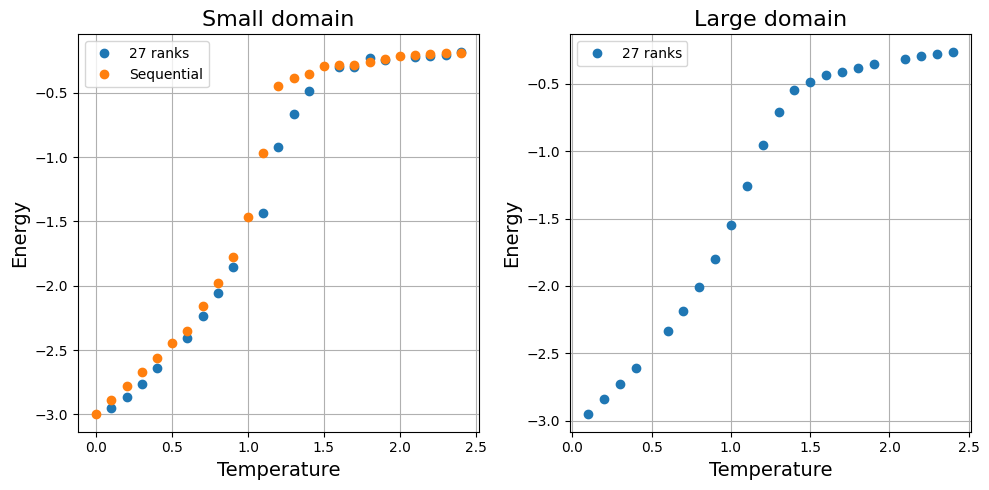
\includegraphics[width=.87\textwidth]{Final_project/Report/energy.png}
    \caption{The total energy per spin in the last iteration of the simulation as a function of temperature.}
    \label{fig:energy}
\end{figure}
\FloatBarrier

\subsection{Magnetization}
The components of the magnetization vector for the whole system is found from the individual spins through

\begin{equation}
    M^{i} = \frac{\sum{S_j^{i}}}{\#spin},
\end{equation}

where $i=x,y,z$ and $j$ runs over each spin. We have also visualized the absolute value of the magnetization in the z-direction of the system as a function of temperature, which can be seen in \cref{fig:mag}. For low temperatures, the magnetization in the z-direction is 1 corresponding to essentially all spins in the system pointing along the z-axis. For higher temperatures, this rises until it becomes zero meaning that all the spins point in random directions. Again, we see that the data from the sequential version follows the same trend as the data from the parallel version of the program as expected.

\begin{figure}[ht!]
    \centering
    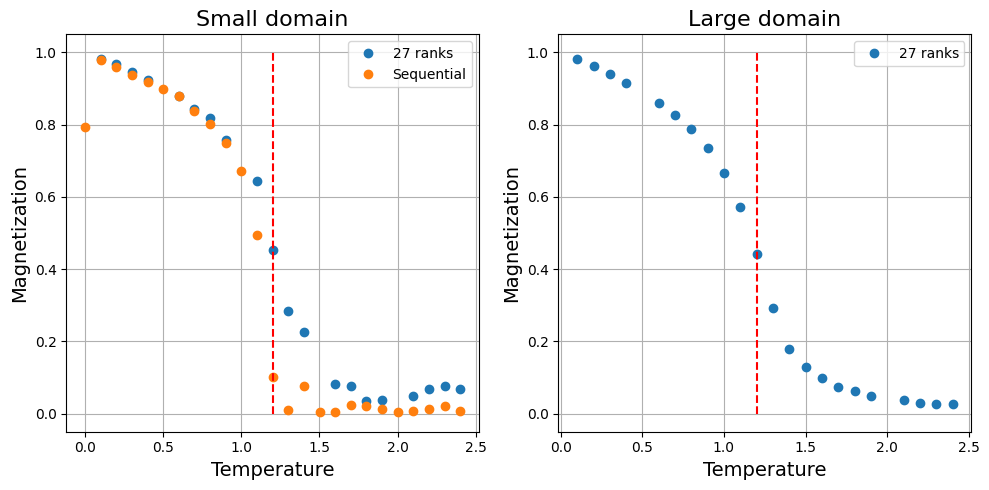
\includegraphics[width=.87\textwidth]{Final_project/Report/mag.png}
    \caption{The absolute value of the total magnetization of the system along the z-axis in the last iteration of the simulation as a function of temperature.}
    \label{fig:mag}
\end{figure}
\FloatBarrier

\subsection{Critical temperature}
The critical temperature of the system is the temperature where the system no longer converges, where order is no longer observed. Since the external B-field applied to the system points in the z-direction, we can find the critical temperature by plotting the z-component of the magnetization of the system as has been done in \cref{fig:mag} and find the temperature at which the system changes from being ordered along the z-axis to being random. The approximate critical temperatures has been read off as $T_{crit} \approx 1.2$, and this is also visualized as a red dotted line in \cref{fig:mag}. The critical temperature appears to be the same for the two system sizes even though the size difference between them ($\#spins=729$ vs. $\#spins=27000$) is quite large. This suggests that the critical temperature is independent of system size.

\subsection{Heat capacity}
From the energy of the individual spins, it is possible to obtain the heat capacity of the system given by

\begin{equation}
    C_v \propto \frac{\left< E^2 \right> - \left< E \right>^2}{\#spin}.
\end{equation}

Hence, we simply need to compute the mean of the squared energy of each spin and subtract the square of the mean energy of the spins and divide by the total number of spins in the system. We have done this for the different temperatures, and the result is plotted in \cref{fig:heat}. It is evident that the heat capacity reaches a maximum just below the critical temperature for both system sizes. And also here, we see that the data from the sequential version of the program follows the same trend as the data from the parallel implementation as expected.

\begin{figure}[ht!]
    \centering
    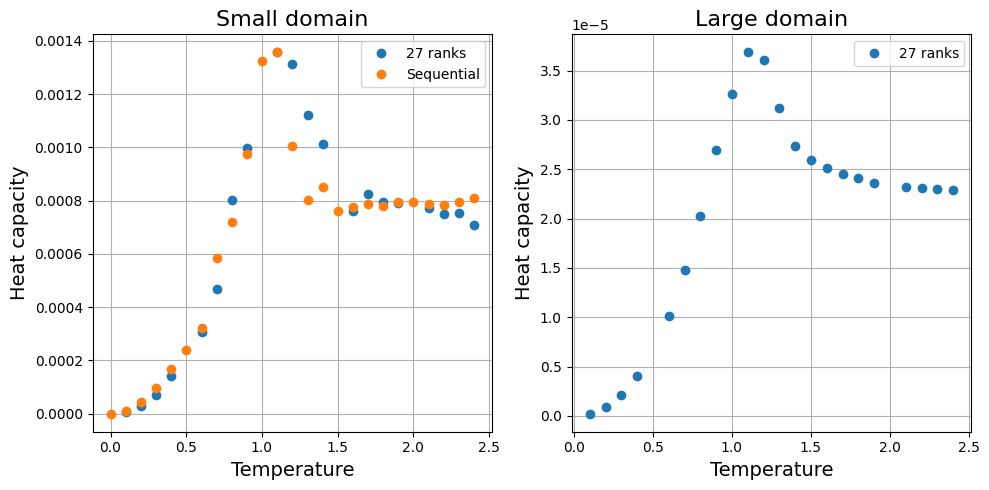
\includegraphics[width=.87\textwidth]{Final_project/Report/heat.png}
    \caption{The heat capacity of the system in the last iteration of the simulation as a function of temperature.}
    \label{fig:heat}
\end{figure}
\FloatBarrier

\section{Scaling}

We have investigated the strong and weak scaling of our parallel implementation. Hence, we have performed benchmarking of both versions of our parallel code and our sequential version in order to compute the speedup of each version of the parallel code compared to the sequential as a function of the number of processors used in the parallel versions. Hence, the speedup is given by

\begin{equation}
    \text{Speedup}(N) = \frac{T_{sequential}(N)}{T_{parallel}}.
\end{equation}

In strong scaling, the size of the problem is kept fixed as the number of processors is increased. In weak scaling, the problem size is scaled linearly to the number of processors.

\subsection{Strong scaling}
To obtain the theoretical parallel fraction of the code according to strong scaling, we have fitted our data to Amdahl's law which is given by \autocite{robeyParallelHighPerformance2021}

\begin{equation}
    \text{Speedup}(N) = \frac{1}{S+P/N} = \frac{1}{1-P+P/N},
\end{equation}

where $N$ is the number of processors, $P$ is the parallel fraction of the code and $S$ is the sequential fraction of the parallel code.
\begin{figure}[h!]
    \centering
    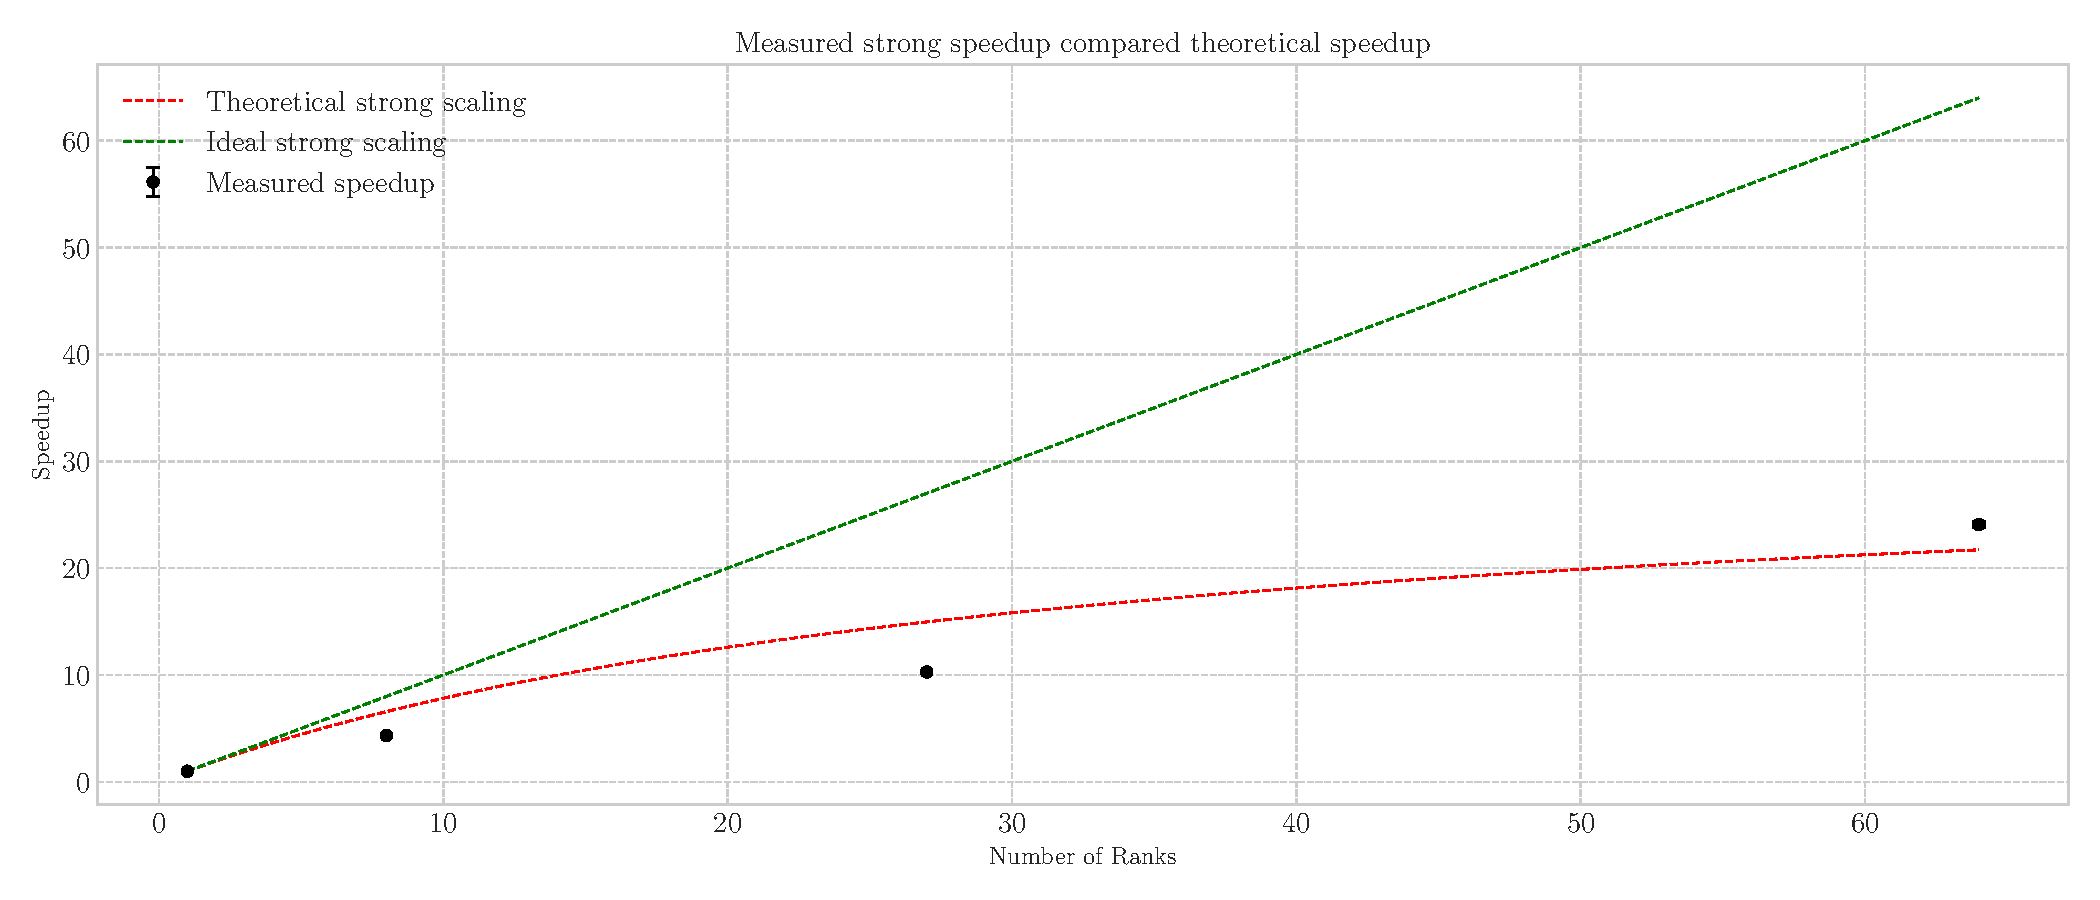
\includegraphics[width=.9\textwidth]{Final_project/Report/strong_scaling.pdf}
    \caption{Plot of strong scaling, with rank \{1, 8, 27, 64\}.}
    \label{fig:strong}
\end{figure}


\subsection{Weak scaling}

To obtain the theoretical parallel fraction of our code according to weak scaling, we have fitted our data to Gustafson's law given by \autocite{robeyParallelHighPerformance2021}

\begin{equation}
    \text{Speedup}(N) = N - S(N-1),
\end{equation}

where $N$ is the number of processors and $S$ is the sequential fraction of the parallel code. Hence, we expect the speedup to scale linearly with the number of processors for weak scaling.
\begin{figure}[h!]
    \centering
    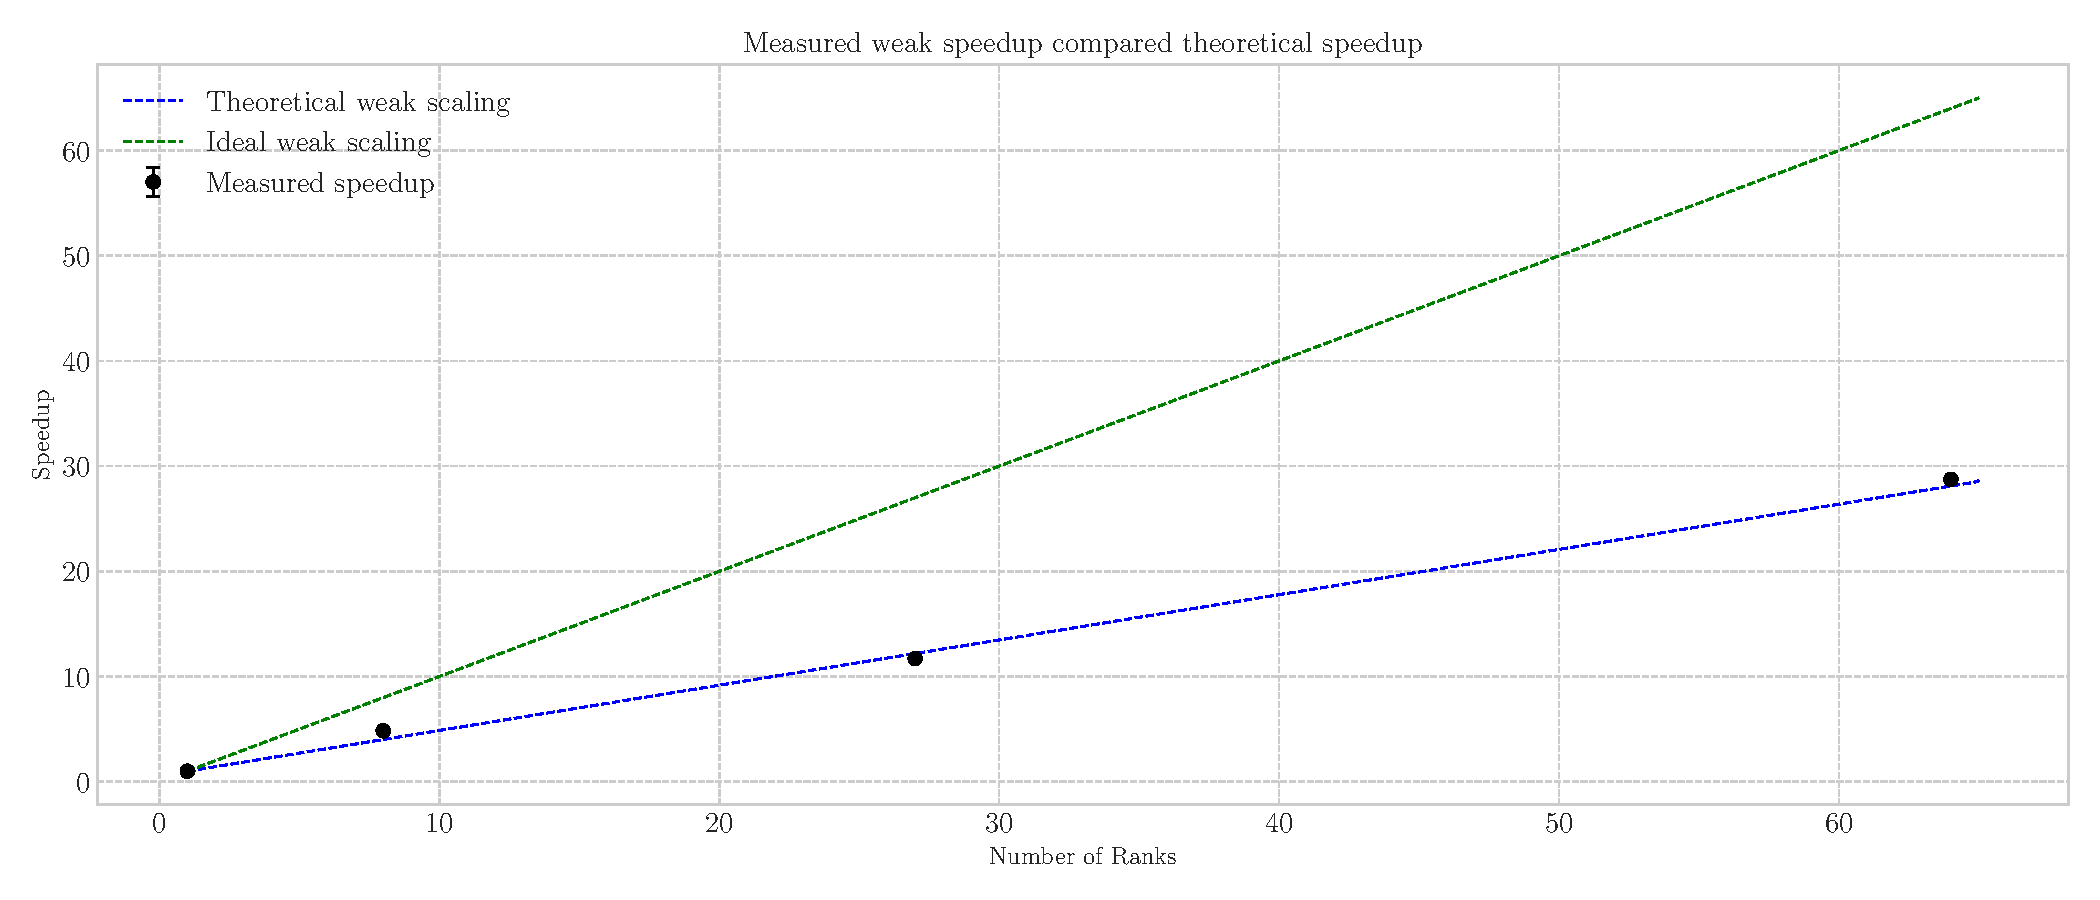
\includegraphics[width=.95\textwidth]{Final_project/Report/weak_scaling.pdf}
    \caption{Plot of weak scaling, with rank \{1, 8, 27, 64\}. Here we varied the system size such that it scaled with the number of ranks.}
    \label{fig:weak}
\end{figure}

In \cref{fig:weak} it is seen that the actual scaling follows the theoretical linear weak scaling quite well. However not nearly close to the ideal speedup.  


\section{Conclusion}

\section{Further ideas}
Due to time constraints not all thinkable optimizations were implemented into the code, and we have had a few ideas which could have helped speed up our implementations even further. 

One of these includes using openMP to do the sending and receiving of ghost cells bewteen neighbouring ranks in our second version. By using hybrid MPI \& openMP, and using the \texttt{MPI\_THREAD\_MULTIPLE} thread level, we could check for messages from, and send messages to, multiple neighbouring ranks at once. This would significantly reduce the overhead introduced by having to check for incoming messages in each iteration, potentially by up to a factor of six if given enough threads. It would also to a smaller degree reduce the overhead introduced by having to send messages to other ranks, as up to three messages potentially have to be sent at once if the flipped spin is in the corner of its domain.

OpenMP would also allow for doing some calculations asynchronously in each iteration. After finding the spin to be flipped multiple different operations could be carried out at once: Determining the current energy in the cell, generating a new direction to be flipped to, and checking if the spin is on an edge so it would potentially need to be sent to neighbours could all be carried out simultaneously with multithreading.

\printbibliography
\appendix
\setcounter{page}{0}
\renewcommand{\thepage}{\roman{page}}
\newpage
\section{Source Code parallel Neighbor\_alltoallw}
\label{sec:source_v1}
\lstinputlisting[language=c++]{../Code/parallel_hsb.cpp}
\section{Source Code parallel Send and receive as necessary}
\label{sec:source_v2}
\lstinputlisting[language=c++]{../Code/parallel_hsb_v2.cpp}

\end{document}